% Chapter 1: Introduction

\section{The Solar-Terrestrial Environment}
The solar terrestrial environment begins with the Sun in the center of the solar system.  The Sun, like most stars, is composed of highly energized plasma that is gravitationally bound together.  This makes it an extremely complex and highly dynamic system that is constantly interacting with the rest of the solar system.  The surface of the Sun is populated with sunspots, dark, relatively cool regions with intense magnetic fields, as well as coronal holes, which are low density areas characterized with a continuous outflow of plasma.  The intense magnetic fields associated with sunspots can break down releasing a large amount of energy and plasma, known as a solar flare.  Planet-sized globs of plasma know as coronal mass ejections (CMEs) can be ejected from the surface, which can be large enough to maintain an internal magnetic field as they travel through the solar system.  The frequency of sunspots and large outbursts of plasma changes with the 22-year long solar cycle.  A large number of Sun spots, high occurrence of fast, dense plasma outbursts, and a highly variably magnetic field indicate solar maximum.  Conversely, solar minimum is characterized by a low Sun spot number and slow and relatively steady outflow.

The Sun interacts with the rest of the solar system through the solar wind, a continuous outflow of plasma that caries the Sun's magnetic field with it.  The solar wind typically has a density around 10 cm\(^{-3}\) at Earth and is traveling away from the Sun at approximately 400 km/s.  However, like the Sun, the solar wind is highly dynamic and these parameters can change drastically over a period of minutes.  CMEs, for instance, create a substantial increase in density and are often proceeded by a shock.  In addition to the outflow of plasma, the solar wind also consisted of the Sun's magnetic field extended into the outer limits of the solar system, called the interplanetary magnetic field (IMF).  Because the Sun has a short rotation period (about 33 days), the IMF gets twisted into a spiral, commonly called the Parker Spiral \citep{Parker1958}.  When the IMF reaches the Earth, the magnetic field is typically oriented at a \(45^\circ\) inclination relative to the ecliptic, but this is highly variable depending on solar wind conditions.

The IMF interacts with the Earth's own magnetic field, the magnetosphere.  Without outside influences, the magnetosphere would be approximately a dipole field, but dynamic pressure from the solar wind causes the Sun facing side to be compressed to 6--10 Earth radii and the rear side to be stretched into an extended tail (hundreds of Earth radii).  Because the solar wind is typically a supersonic flow, a bow shock forms on the dayside of the magnetosphere.  The heated and compressed solar wind plasma created by the bow shock is known as the magnetosheath.  The magnetopause is the actual boundary between solar wind plasma in the magnetosheath and magnetospheric plasma.  However, the magnetosphere is not fully closed.  At the magnetopause, magnetic reconnection can occur between the IMF and the Earth's magnetic field creating open field lines.  Magnetic field lines originating from the Earth are then directly connected to the Sun through the solar wind, which consequently allows highly energized solar particles to enter the magnetosphere.  Open field lines tend to occur around the Earth's polar caps, making these regions particularly interesting to study due to very complex behavior and coupled interactions between the Earth and the Sun.

Closer to the Earth's surface, the magnetosphere also interacts with the Earth's ionosphere, a layer of partially ionized plasma in the upper atmosphere.  The interaction between charged particles in the ionosphere with magnetic field lines from the magnetosphere couples these two regions and creates non-trivial dynamics.  In addition, highly energized charged particles from the solar wind travel along open field lines and collide with both ions and neutral particles in the ionosphere, creating the aurora at high latitudes.  Below the ionosphere, the thermosphere consists mostly of neutral particles, however neutral winds can influence the ionosphere through viscous interactions along the lower boundary.  All of these regions contain incredibly complex dynamics and are additionally all interconnected, creating a complicated system that is extremely challenging to describe completely.  

\section{The Earth's Ionosphere}
\label{sec:ionosphere}
The Earth's ionosphere is a region of the upper atmosphere that ranges approximately between 50--1000 km in altitude where neutral gases have been excited so that they are partially ionoized, resulting in free electrons and ions mixed with neutral particles.  Two conflicting processes occur in the ionosphere to create a peak in electron density, commonly referred to as the Chapman Layer \textbf{CTIE CHAPMAN?}.  Solar illumination and particle precipitation ionize neutrals, and the density of ions increase as altitude decreases because there are more neturals available to ionize.  However, below a certain point, the concentration of ions becomes large enough that recombination into neutral particles becomes a substantal factor, reducing the ion density.  The exact altitude where this density peak occurs is variable with time of day, location, season, and solar cycle.  A profile of how electron density changes with altitude is shown in Figure \ref{fig:densprofile}.

\begin{figure}
	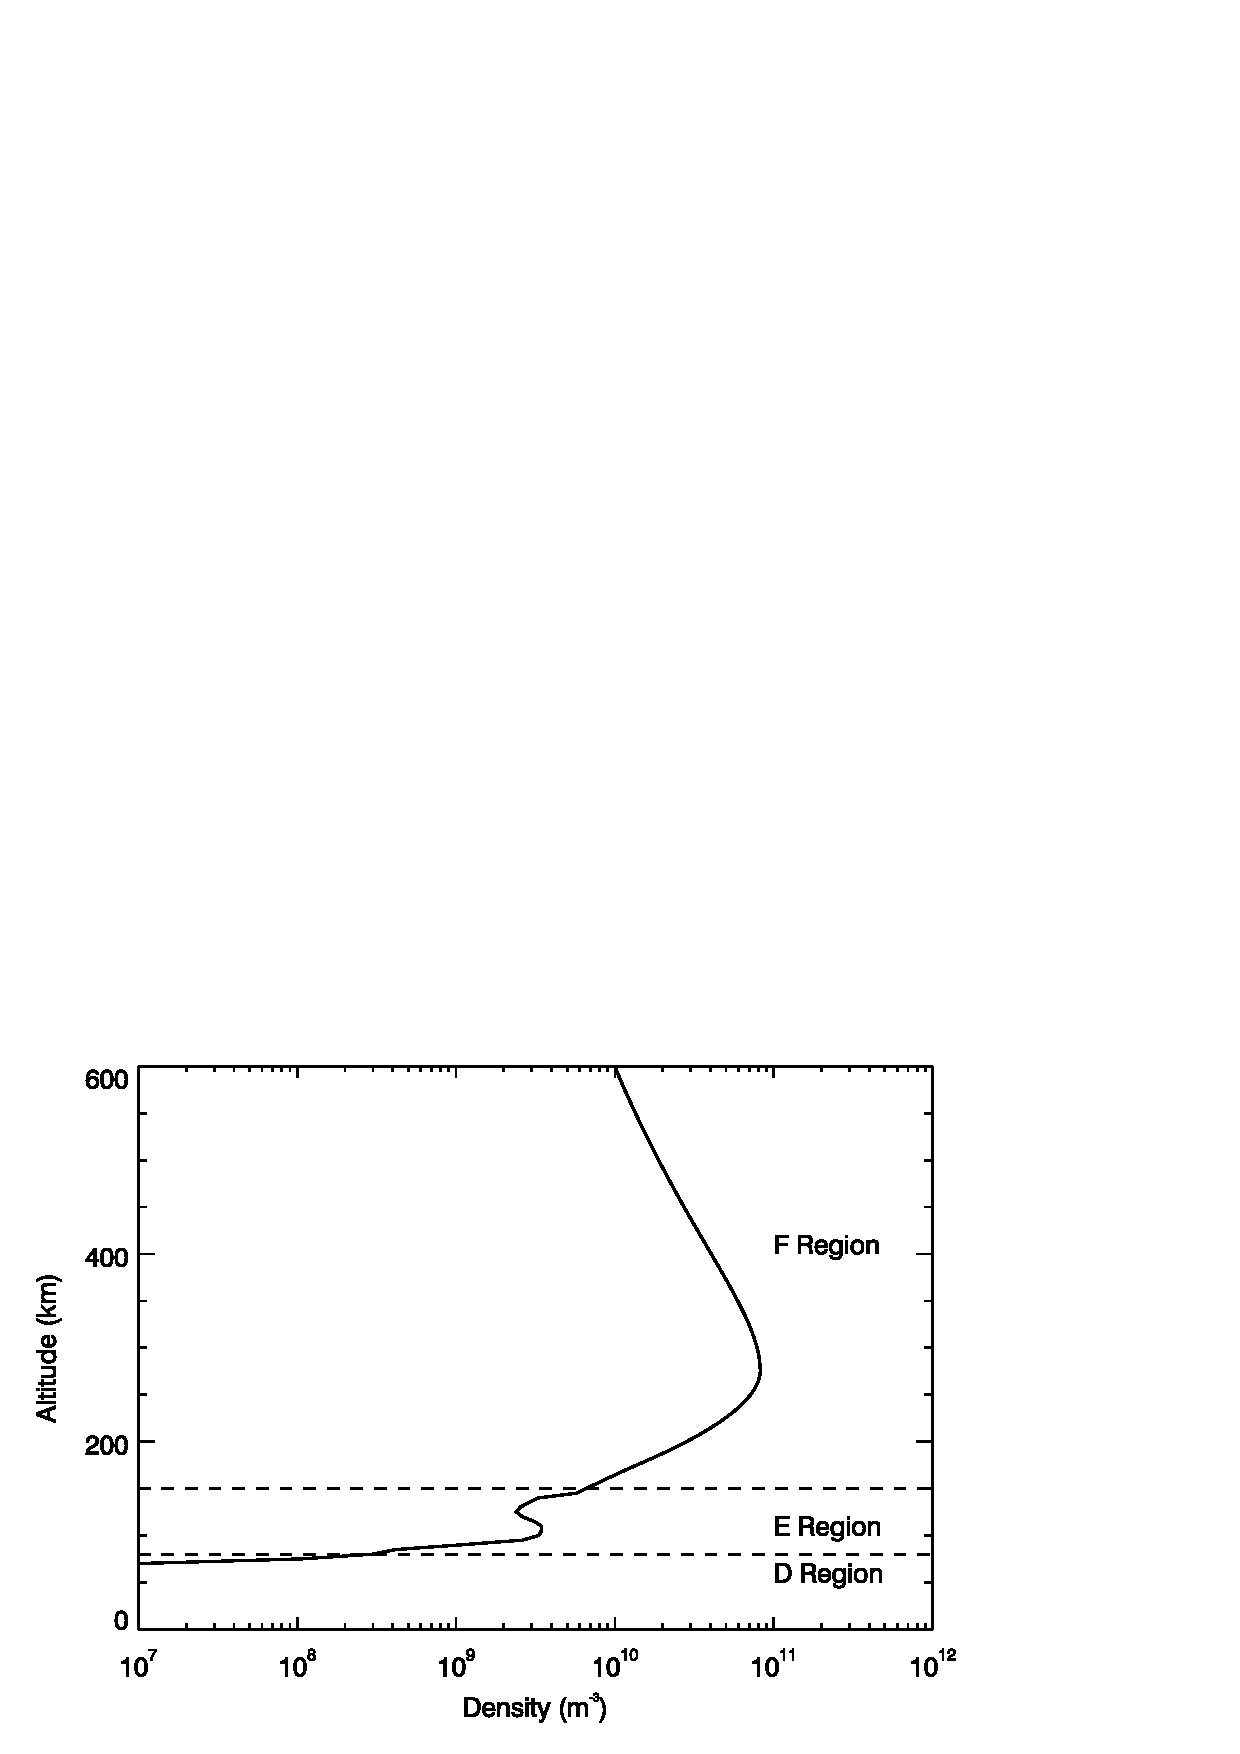
\includegraphics[width=\textwidth]{densprofile.pdf}
	\caption{Altitude profile of electron density throughout the ionosphere.  Typical ranges of the D, E, and F regions are identified.}
	\label{fig:densprofile}
\end{figure}

Above 50 km, the primary neutral particles are atomic oxygen, O, molecular oxygen, \(O_2\), and molecular nitrogen, \(N_2\).  Common ions at these altitudes are therefor mostly composed of oxygen and nitrogen, \(O^+, NO^+, O_2^+, N_2^+\), but hydrogen, \(H^+\), can contribute as well \citep{Kelley2009}.  In the ionosphere, neutral densties are typically several orders of magnitude higher than ion densities, however even a small number of charged particles changes the behavior of the region dramatically.  Because there are so many different ion species, plasma density is usually discussed simply in terms of electron density.

\subsection{Ionosphere Regions}
\label{sec:ionosphere_regions}
The ionosphere is typically divided into three region, Figure \ref{fig:densprofile}.  The D region is located between 80 and 90 km in altitude and typically only exists in the daytime when the ionosphere is sunlit.  The E region typically exists between 90 and 120 km with a density peak between 105 and 110 km, depending on factors such as time of day and season.  Above 120 km is considered the F region, which has a density peak between 300 and 400 km.  The F region can actually have two peaks under some daytime conditions, notated as the F1 peak and the F2 peak.  The locations and peak densities of each of these regions is highly variable both diurnally and seasonally.  In Figure \ref{fig:densprofile}, the daytime profile is shown with the solid line next to a nighttime profile with a dashed line.  Note that night electron densities are lower at all altitudes due to the lack of photoionization durring nighttimes.  In addition, the F-region peak moves to higher altitudes at night.

Because the concentrations of ions and neutral particles changes with altitude, each of these regions have distinct plasma physical properties that make them unique and change how plasma structuring forms.  The main change that occurs is wether the the large-scale motion of a particle is controlled more by the magnetic field (the particle is magnetized) or by collisions with other particles (collisional).  This can be determined by comparing the collision frequency, \(\nu_\alpha\), to the gyrofrequency, \(\Omega_\alpha\), of a particular species.  If \(\Omega_\alpha \gg \nu_\alpha\), the particle completes many gyrations between each collision, so its motion is determined mostly by the magnetic field and it is magnetized.  If \(\nu_\alpha \gg \Omega_\alpha\), the particle collides with other particles much more often than it complete a gyration, so it is considered collisional.  The gyrofrquency is dependent on the mass and charge of the particle and the strength of the magnetic field, \(\Omega_\alpha = q_\alpha B/m_\alpha\), so is roughly constant through the ionosphere because the magnetic field strength does not change much through these altitudes.  The collision frequency depends on the density of a species relative to the density of all other species in the plasma and can be calculated from a series of complicated expressions \citep{Schunk1980,Schunk2009}.  In the E region, \(\Omega_e \gg \nu_e\), so electrons are magnetized.  However, the motion on ions is dominated by collisions between ions and neutrals (\(\nu_i > \Omega_i\)), so ions in the E region are considered collisional.  In the F region where the neutral density is much lower, both ions and electrons are magnetized, \(\Omega_\alpha \gg \nu_\alpha\).  These differences in how charged particles move vary the conductivity and can strongly impact how plasma waves develop, which will be discussed further in Section \ref{sec:lit_theory}.

\subsection{Plasma Structuring in the Polar Ionosphere}
\label{sec:polar_structure}
The polar ionosphere is a particularly interesting and dynamic region due to the presence of the magnetic poles and open field lines to the solar wind.  Plasma structuring can occur as variations in density, velocity, or temperature, but the main focus of this work will be density perturbations, often called irregularities.  Density irregularities in the polar cap can occur on scales ranging from thousands of kilometers to less than a centimeter \citep{Tsunoda1988}.  Large-scale plasma irregularities are typically considered to be any density structuring on the scale of 1 -- 1000 km.  Some common examples are polar patches, polar holes, and sun-aligned arcs.  Polar patches are large density enhancements (usually at least twice the background plasma density) that travel across the polar cap with the background convection.  Polar holes are plasma density depletions that typically occur in the F region slightly poleward of the auroral oval.  Sun-aligned arcs are large density forms that stretch across the polar cap along the sun-earth line.  They are very narrow and often characterized by large and complex velocity shears on either side of the arc.

Intermediate-scale structuring typically ranges from 100 m -- 1 km.  This is also referred to as scintillation-causing structuring and is responsible for many of the negative space weather effects that are observed on Earth.  Radio signal scintillation through the ionosphere changes the phase and amplitude of the original signal, which can effect the ability that satelites have to communicate with ground recievers.  This can cause communication blackouts or introduce large errors into GPS calculations, effecting navigation.  Because communication and navigation technology is implemented in both every day civilian life as well as government and military intrests, the effects of this kind of signal scintillation can be far reaching.

Small-scale structuring is generally considered to be all irregularities less than 100 m.  Although the effects of these scale sizes on navigation and communication systems are minimal, they can be the easiest to study because of large data sets collected from high frequency ionospheric radars globally for several decades (discussed further in Section \ref{sec:superdarn}).  The irregularity sizes presented here are rough categories only and a high degree of coupling between different scales is generally considered reasonable.  For instance, large-scale structures such as polar patches may very well have internal intermediate- or small-scale structuring.  Some kind of turbulent cascade is often assumed to connect these different scales, but because various instruments or techniques usually only observe structuring on a particular scale, it is difficult to find direct evidence of this or how exactly it occurs.

\section{Observational Techniques and Models}

%Figures
%- Map of radars (Northern and southern hemisphere)
%- Example convection map
%- Example ISR profile
%- Example MSISE profile?
%- Example of IGRF?
%- How does radar work diagram
%- Pulse sequence diagram

\subsection{Coherent Scatter Radars}
\label{sec:csr}
Coherent Scatter Radars (CSR) have been used to study the ionosphere for the last half century.  The radar transmits a radio wave, which can reflect off plasma structuring in the ionosphere, and then be detected by the recieving antennas.  The time difference between when the signal was transmitted and when it was detected and the power and phase of the returned signal can then be used to determine local characteristics of plasma irregularities.

There are three measurements typically made by CSR systems: backscatter power, line of sight (LoS) velocity, and spectral width.  Backscatter power is the power of the retuned signal that the radar's recievers detect.  Typically, a threshold is selected for the minimum power acceptable for a return to be considered an actual signal instead of background noise.  LoS velocity is the component of the total plasma drift velocity that is measured along one beam of a radar.  Because radars measure velocity through the doppler shift of backscatter, only the component of the velocity vector that is along the radar beam can be measured.  Spectral width represents the width of the doppler power spectrum and can determine some of the characteristics of irregularities \citep{Greenwald1985}.

CSR systems typically operate by transmitting pulses instead of continuously.  This allows the distance between the radar and the target to be found (based on the time difference between when the pulse is transmitted and received).  The size of the range gate is determined by the length of a radar pulse, Equation \ref{eqn:range_gate}.
\begin{equation}
	\label{eqn:range_gate}
	\Delta r = \frac{c\Delta t}{2}
\end{equation}
Longer pulses result in larger range gates, resulting in poorer spatial resolution.

When the radar transmits continuously, backscatter will be received, but because it is impossible to know when that signal was transmitted, the difference in time between transmission and receiving cannot be used to calculate how far away the backscatter volume is.  Conversly, if the radar only transmits a pulse of a certain length of a certain length and then "listens" for its return, the time between transmission and return is known and the distance the pulse traveled can be calculated and therefore the location of the backscattering volume.  However, using this simple single-pulse method another pulse cannot be transmitted until the first pulse returns, limiting the temporal resolution that can be achieved.  This can be improved by using a multipulse scheme, which will be discussed below.

A short time between pulse returns is nessisary to allow dopler velocities to be calculated, particularly at long ranges.  The maximum dopler shifted frequency that can be observed by a radar is the Nyquist frequency, which is equivilent to half the sampling frequency, Equation \ref{eqn:nyquist}.
\begin{equation}	
	\label{eqn:nyquist}
	f_n = \frac{f_s}{2}
\end{equation}
Radars operating in single-pulse mode have a very limited sampiling frequency, as described above, particularly at long ranges where the pulse must travel a long distance.  This severely limits the dopler shift that can be measured, which places an upper limit on the LoS dopler velocity that can be calculated with this technique.  For an ionospheric radar observing a structure 2000 km away, it would take about 13 ms for a signal traveling at the speed of light to travel to the the structure and back to the radar, wich corresponds to a sampling frequency of \(f_s = 75\) Hz.  The Nyquist frequency is then \(f_n = 37.5\) Hz, which corresponds to a maximum measurable Doppler velocity of \(\sim550\) m/s.  Flows in the ionosphere have been known to exceed 1000--2000 m/s, so single pulse sampling is insufficient for these purposes.

%BENIFITS OF MULTIPULSE: Ponomarenko and Waters, 2006
Instead of waiting for each individual signal to be recieved before transmitting the next, ionospheric radars typically employ a multipulse mode. In a multipulse mode, the radar transmits a series of pules with different time intervals or lags between them.  This can introduce complications when backscatter from different pulses at different ranges is received by the radar at the same time, referred to as cross-range interference, but these effects can be mitigated using correlation techniques.  The smallest lag between two pulses is known as the multi-pulse increment, \(\tau\).  All other lags are integer multiples of \(\tau\), which allows the calculation of the corresponding lags of the complex autocorrelation function (ACF).  The ACF is used to find the spectral characteristics of the backscatter, from which the LoS velocity, spectral width, and backscatter power can be obtained.  Overall, multi-pulse techniques are generally considered far more appropriate for ionospheric studies than single pulse \citep{Farley1972,Greenwald1983,Greenwald1985,Barthes1998,Ponomarenko2006}.

The first instance of CSR being used to study plasma density structures in the ionosphere was the Scandanavian Twin Auroral Radar Experiment (STARE) in the 1970s and 1980s.  STARE consisted of two very-high frequency (VHF) radars with overlapping FoVs that were designed to measure FAIs in the E region of the ionosphere \citep{Greenwald1997}.  The advantage of two radars with overlaping FoVs was the ability to observe the same structures from two different orientations.  Because each radar can only measure the LoS velocity of a structure, two simultanious observations from different directions allows two different velocity vecotor compontents to be found, and hense the total velocity vector can be calculated.  This technique is still commonly used with CSR system.

%- How to measure power, spectral width, LoS velocity
%	- What are these things?
%- Hanuise, 1993b
%- Baker, 1995

\subsubsection{SuperDARN}
\label{sec:superdarn}
The Super Dual Auroral Radar Network (SuperDARN) is a global network of HF CSRs that was designed to measure small-scale plasma structuring in the ionosphere and map the global plasma convection.  The network currently consists of about 35 operational radars between the northern and southern hemispheres distributed at mid-, high-, and polar latitudes, Figure \ref{fig:superdarnmap}.  Following the STARE experiment \citep{Greenwald1978}, the first HF ionospheric radar was built in Goose Bay, Canada in 1983, which would become the first of the SuperDARN radars \citep{Greenwald1985}.  

\begin{figure}
	\includegraphics[width=\textwidth]{superdarnmap.pdf}
	\caption{FoVs of all operational SuperDARN radars in both the northern (left) and southern (right) hemispheres.  Polar latitude radars are shown with the red outlines.  The radars at Rankin Inlet (northern hemisphere) and McMurdo Station (southern hemisphere) are shaded in red because these two instruments are particularly important in the following studies.  Lines of constant magnetic latitude are shown in yellow at \(\Lambda = 40\deg, 60\deg, 80\deg\) in the northern hemisphere and at \(\Lambda = -40\deg,-60\deg,-80\deg\) in the southern hemisphere.}
	\label{fig:superdarnmap}
\end{figure}

It is nessisary to use HF radars to study ionsospheric structures in the polar cap because the magnetic field is close to vertical and in order for the radar beam to meet the perpendicularity condition to observe FAIs, the beam must be refracted through a dense ionosphere.  VHF radar beams are not refracted enough in the polar cap and the beam will pass through the ionosphere without reflecting off any FAIs.  SuperDARN radars operate at a nominal 8--20 MHz frequency, which, according to the Bragg scatter equation for backscatter, corresponds to observing decameter-scale plasma waves.  Each radar consists of 16 independent transmit and recieving antennas.  Beams are electronically steerable and most radars have between 16 and 24 beams in normal operation mode, each beam being \(3.25\deg\) in azimuth.  Each beam consists of 75--100 range gates, which are generally either 15 km or 45 km in length \citep{Chisham2007}.  SuperDARN radars were originally designed to used a 7 pulse ACF \citep{Farley1972,Greenwald1983,Greenwald1985}, however since 2011, most radars have begun using an 8 pulse sequence.   The multi-pulse increment, \(\tau\), is 2400 \(\mu\)s, which corresponds to a Nyquist frequency of about 200 Hz, small enough to measure plasma drift velocities up to 3000 m/s.  The spectral characteristics of backscatter of recovered from the ACF using the FITACF algorithm \citep{Ponomarenko2006}.

One of the original purposes of SuperDARN was to produce maps of the plasma convection patterns in the polar caps using 2D velocity vectors.  Originally this was accomplished by considering two radars with overlapping FoVs.  If both recieved backscatter from the same scattering volume, two LoS velocities could be found for that scattering volume, which could be combined to find a 2D velocity vector \citep{Ruohoniemi1989}.  The modern method for creating convection maps involves taking all data recorded by all radars in a particular hemisphere and finding the best fit to a 2D ionospheric electrostatic potential using Legendre functions \citep{Ruohonomiemi1998}.  For convection maps, only data from the F region is considered.  If there is not enough velocity data to confine the fit sufficiently, the measured data points are supplimented with a statistical model based on solar wind IMF conditions \textbf{CITE MCWILLIAMS???}.

Because convection maps require data covering as wide a range of magnetic local time sectors as possible, SuperDARN radars are continuously operational, usually in a common mode.  This creates a vast database of high-quality measurements of small-scale FAIs, which is very useful for other studies on irregularity occurrence and plasma structuring.

\subsection{Incoherent Scatter Radar}
\label{sec:isr}
Similar to CSRs, incoherent scatter radars (ISRs) are ground based radars that are used to probe the ionosphere.  However, they use a fundamentally different technique to observe structuring, which allows them to measure different things than CSRs.  Where as CSRs receive backscatter from large, "coherent" density structures in the ionosphere, ISRs operate by radar beams scattering due to the random thermal motion of electrons in the ionosphere.  The radar receivers then detect a spectra of frequencies with different power.  Analysis of this spectra will reveal the plasma frequency, and hence, the electron density, electron and ion temperature, and LoS velocity \citep{Gordon1958}.

The first ISR was built in Arecibo, Puerto Rico in 1958.  Since then, at least 8 other ISRs have been deployed around the world at equitoral, mid-, and high-latitudes.  The most recent advancement has been the development of Advanced Modular Incoherent Scatter Radars (AMISR), of which there are currently three in use, one at the Poker Flat Rocket Range, just north of Fairbanks, AK and two in Resolute Bay, Canada.  The advantage of these new systems is that they are electronical steerable, unlike older ISRs which consisted of a large dish that had to be moved manually to change the beam direction.  This allows beams to be transmitted in many different directions at a very high time cadence, giving the radar the capability to make measurements in multiple directions almost simultaniously.  This is very important for creating 2D maps of ionospheric conditions and tracking how they change in time.

\subsection{IRI Model}
\label{sec:iri}
Models can be useful tools for establishing the context of experimental measurments, especially in a global sense.  In particular, it is impractical to achieve full global coverage of all instruments, so models can be a useful way to fill in the gaps.  There are two main categories of models.  Theoretical models are based on first principles and global pictures are often found by running large computer simulations based on these first principles.  They can help give insight as to what causes specific phenomena because the process can be followed beginning to end.  Empirical models are based purely on measured data.  These can potentially be more accurate because they should replicate real measurments, but they also do not give any insight into how the system got to its ending state.  In addition, empirial models are often heavily averaged.

The international reference ionosphere (IRI) is an empirical model of the Earth's ionosphere.  It was originally created in 1969 as a joint effort between the Comittee on Space Research (COSPAR) and the International Union of Radio Science (URSI) and has been periodically updated since then \citep{Rawer1978}.  The current version is IRI-2012 \citep{Bilitza2014}, which is used throughout the work done here.  It can be accessed either as an online module or by downloading and running the FORTRAN source code, both of which are available from the International Reference Ionosphere page on the NASA website (http://iri.gsfc.nasa.gov/).

The IRI model can produce outputs of electron density, temperatures of electrons, ions, and neutrals, ion composition (O+, H+, He+, O2+, NO+, N+), and total electron content (TEC).  The model requires the input of a location (latitude, longitude, and altitude) and time (year, date, and time).  Internally, the model has the additional capability of producing profiles in any of the input parameters.  This is particularly significant for height profiles, and allows the peak heights and densities of the E and F region to be calculated.

%- Empirical model of the global ionosphere
%- Parameters that can be calculated
%- How is it available?
%	- Online
%	- FORTRAN source code
%- Biltza, 1990

\section{Theory and Observations}
Much work has been done over the past several decades to try to understand the complicated picture of plasma structuring in the polar cap, both from theoretical analysis of plasma dispersion relations, simulations of plasma dynamics, and observations of plasma structuring using a variety of instruments.

\subsection{Theory and Simulations}

Polar patches are large regions of enhanced plasma density in the polar F region \citep[][e.g.]{Weber1984,Buchau1983}.  They are know to emerge on the dayside and then propagate with the background plasma convection across the polar cap to the nightside, where they either disintegrate or recombine with enhanced-density plasma in the auroral oval \textbf{CITE SOMETHING}.

There have been at least 6 mechanisms proposed for how polar patches form on the dayside.
\begin{enumerate}
	\item Discrete changes in solar wind parameters, usch as IMF, density, speed, and pressure \citep{Sojka1994}
	\item Average flow patterns varying in time \citep{Anderson1988}
	\item Transient magnetopause reconnection \citep{Lockwook1992b}
	\item Plasma production by cusp particle precipitation \citep{Rodger1994,Millward1999}
	\item Plasma flow jet channels that cut continuous streaches of plasma into segments 	\citep{Valladares1998}
	\item Alfven wave coupling \citep{Prikryl1999}
\end{enumerate}
Although particle precipitation has been shown to create enhanced plasma density in the cusp region \citep{Roger1994}, it is unreasonable for this mechanism to account for the largest density enhancements observed in polar patches.  These high densities must originate from the resivor of solar illuminated plasma on the dayside.  Additionally, a mechanism is still required to separate patches from the cusp region.  High speed flow channels can "cut" segments off of a tongue of high-density plasma that has been pulled into the polar cap by convection \citep{Valladares1994,Valladares1998}.  Models have also shown changing large scale convection patterns quickly in time does produce density structures similar to patches \citep{Anderson1988}.  However, the mechanism that seems to be dominant for the majority of polar patches observed is transient magnetic reconnection \citep{Carlson2012}.

In order to discuss patch formation by transient magnetic reconnection, it is important to first understand the steady-state ionospheric convection patterns in the polar cap and how they relate to the magnetosphere.  Figure \ref{fig:magnetosphere} is a schematic of how the IMF, magnetosphere, and ionosphere are all interconnected.  In general, magnetic field lines in the magnetosphere can either be closed, meaning they connect only the north and south pole of the earth, or open, when one of the ends of the field lines originates from the sun such that the field line is connected directly to the IMF.  The polar cap boundary is generally defined as the border between open and closed field lines, shown by the dark line in figure \ref{fig:magnetosphere}.  By Faraday's Law, the total EMF around the polar cap boundary is equal to the rate of change of magnetic flux, equation \ref{eqn:pc_imf}.  In the polar cap, the magnetic field strength is relatively constant at around \(5\times 10^-5\) T, so any changes in magnetic flux must be due to changes in the polar cap area, \(A_{pc}\) due to the polar cap boundary expanding or contracting \citep{Lockwood1992a}.
\begin{equation}
	\label{eqn:pc_imf}
	-E = \frac{d\Phi_B}{dt} = B\frac{dA_{pc}}{dt}
\end{equation}
Magnetic reconnection often occurs on both the dayside and nightside of the magnetosphere, changing the amount of open magnetic flux, so the polar cap boundary can be highly dynamic.

Magnetic reconnection between the IMF and the Earth's magnetosphere occurs along the X-line on the dayside magnetopause (blue line in figure \ref{fig:magnetosphere}).  The X-line in the magnetopuase can be mapped along the magnetic field lines to the ionosphere, where it is referred to as the merging gap (pink line in figure \ref{fig:magnetosphere}).  During reconnection events, the merging gap moves equatorward as the open magnetic flux into the polar cap increases \citep{Lockwood1992a}.  In addition, the potential along the X-line also gets mapped the the merging gap, assuming there is minimal drop in potential along the magnetic field lines \citep{Lockwood1992b}.  The combination of these two effects results in flux being transferred across the boundary at a rate equal to the applied voltage  along the X-line and hence plasma flow across the merging gap \citep{Lockwood1992b}, as seen in figure \ref{fig:patch_formation}.  As the reconnection event continues, the flow across the merging gap creates a convection pattern, which starts to pull high density plasma from the dayside into the polar cap.  If this continues consistently, eventually it can create a "tongue" of high-density plasma stretching between the dayside merging gap and the center of the polar cap, often called the tongue of ionization.  However, when the reconnection burst ends, the merging gap begins to relax back towards the polar cap and brings the dense plasma with it, figure \ref{fig:patch_formation}.  Before the flow stops completely, the patch "pinches off" of the ionization tounge and becomes an isolated island of high density plasma in the polar cap.  The merging gap returns to its original position and the entire process can repeat with the next reconnection event.  A series of reconnection events will create a string of isolated polar patches propigating through the center of the polar cap \citep{Lockwook1992b}.

Plasma structuring occurs in the ionosphere when conditions are such that wave growth occurs.  Because different background conditions change factors such as the density of both neutrals and ions, the magnetic field strength, and so forth, the collison frequency, gyroradii, and ion inertial effects change at different altitudes.  This causes a variety of different instability mechanisms to be operational depending on the background conditions.  The Farley-Buneman instability (FBI), or the modified two-stream instability tends to be a major factor in the E region where ion inertial effects are high \citep{Farley1963,Buneman1963}.  Also operational in the E region but more dominant at higher altitudes is the gradient-drift instability (GDI) \citep{Simon1963,Hoh1963,Linson1970}.  When GDI is stable, wave growth can still occur sometimes along the magnetic field, which is known as the current-conductive instability (CCI).  Additionally, there are shear-driven processes, known as the Kelvin-Helmholtz instability (KHI) \textbf{CITE???}.

In the polar F-region ionosphere, GDI is typically considered the dominant structuring process \citep{Weber1984,Cerisier1985,Basu1988,Tsunoda1988}.  GDI is operational when high-density purturbations in the plasma move to regions of lower background density and low-density purturbations in the plasma move to regions of higher background density, such that the wave amplitude grows relative to background conditions.  As plasma drifts and carries irregularities with it, the ions in high density perturbations lag behind the electrons and create a purturbed electric field.  This purturbed electric field combined with the background magnetic field causes the density perturbations to \(\vec{E}\times\vec{B}\) drift.  If the drift causes high and low density perturbations to move as desribed above, the instability is operational and the perturbations grow.  If instead high density perturbations drift into regions of higher background density and low density perturbations drift into regions of lower background density, the wave is damped.

Some of the first 1D investigations of the linear GDI growth rate found that it can be described by a simple expression involving the plasma drift velocity, \(V_E\), and the gradient scale length, \(L\) \citep{Simon1963,Hoh1963,Linson1970}.
\begin{equation}
	\label{eqn:gdi_old}
	\gamma = \frac{V_E}{L}
\end{equation}
This expression is only valid if the density gradient is in the same direction as the plasma drift velocity and wavevector direction is not considered.  The results of \citet{Keskinen1982,Keskinen1983} do consider the wavevector, \(\vec{k}\), to some extent, but still assume a general relationship between density gradients and plasma drift \citep{Tsunoda1988}.
\begin{equation}
	\label{eqn:gdi_80s}
	\gamma = \frac{k_y}{k}\frac{\vec{k}\cdot\vec{V}_E}{kL}
\end{equation}
The directional dependance of GDI has been shown to be significant, such that the growth rate can actually change signs (determining whether wave growth or damping occurs) with different wavevector directions, so it is important to consider this factor \citep{Makarevich2014c}.  In addition, these expressions are only applicable in a particular altitudinal regieme, usually the F region.

Recently, a new expression has been introduced that considers an arbitrary altitude, wavevector, and density gradient within the ionosphere, which allows FBI, GDI, an CCI to be considered with a single dispersion relation \citep{Makarevich2016a}.
\begin{equation}
	\label{eqn:gdi_Mak16}
	(H_i-H_e)\omega = (H_i\vec{V}_{e0}-H_e\vec{V}_{i0})\cdot\vec{k}+(C_i-C_e)H_eH_i
\end{equation}
As before, \(\vec{k}\) is the wavevector and \(\vec{V}_{\alpha 0}\) is the velocity of species \(\alpha\).  The species \(\alpha\) is given by either \(i\) for ions or \(e\) for electrons.  The other quantities in equation \ref{eqn:gdi_Mak16} are not standard and described below.
\begin{equation}
	H_\alpha = S_\alpha F_\alpha + D_\alpha^{-1} F_\parallel \quad\quad\quad
	C_\alpha = \frac{T_\alpha}{m_\alpha \Omega_\alpha}
\end{equation}
\begin{equation}
	F_\alpha = i k_\perp^2 D_\alpha + \vec{G}\cdot\vec{k}_\perp D_\alpha + \vec{G}\cdot\vec{k}\times\uvec{b} \quad\quad\quad
	F_\parallel = i k_\parallel^2 + \vec{G}\cdot\vec{k}_\parallel
\end{equation}
\begin{equation}
	S_\alpha = \frac{1}{1+D_\alpha^2} \quad\quad\quad
	D_\alpha = -\frac{i}{\Omega_\alpha}(\omega-\vec{k}\cdot{V}_{\alpha 0})+r_\alpha
\end{equation}
The quantity \(r_\alpha\) is the ratio of the collision frequency to the gyrofrequency of a particular species, given by \(r_\alpha = \nu_\alpha/\Omega_\alpha\).  

It is useful to express Equation \ref{eqn:gdi_Mak16} in the following equivalent form by defining additional terms.
\begin{equation}
	\label{eqn:gdi_Mak16_alt}
	\left(D_i-D_e\right)\omega = \vec{V}_d\cdot\vec{k}\left(\frac{Z_2}{Z_1}\right) + \left(D_i\vec{V}_{i0}-D_e\vec{V}_{e0}\right)\cdot\vec{k}+(C_i-C_e)k_{\perp}^2\left(\frac{Z_3}{Z_1}\right)
\end{equation}
In the F region where background plasma motion is dominated by electric fields perpendicular to the magnetic field, the differential plasma velocity, \(\vec{V}_d\), can be described as 
\begin{equation}
	\label{eqn:gdi_Mak16_Vd}
	\vec{V}_d = \vec{V}_{e0}-\vec{V}_{i0} = (r_i-r_e)\left[s_es_i(1+\psi)\left(R\vec{V}_E-\frac{\vec{E}}{B}\right)\right]
\end{equation}
where, \(s_\alpha = (1+r_\alpha^2)^{-1}\).  Additionally,
\begin{equation}
\label{eqn:gdi_Mak16_Z}
\begin{split}
	Z_1 = i(1+Y)+a+Rb+ycK \quad\quad\quad 
	Z_2 = R(i+a)-b \quad\quad\quad\quad\quad\quad\\
	Z_3 = -\frac{\Psi(i+a)^2}{1+\Psi}-Rb(i+a)+\frac{b^2}{1+\Psi}-iy(y-ic)\left[\left(K+1-\Psi^{-1}\right)(i+a)+Rb\left(1-\Psi^{-1}\right)\right]\\+Ky^2(y-ic)^2
\end{split}
\end{equation}
and
\begin{equation}
\begin{split}
	a& = \frac{\vec{G}\cdot\vec{k}_\perp}{k_\perp^2} \quad\quad\quad
	b = -\frac{\vec{G}\cdot\vec{k}\times\uvec{b}}{k_\perp^2} \quad\quad\quad
	c = \frac{\vec{G}\cdot\vec{k}_\parallel}{k_\perp k_\parallel} \\
	\Psi = -D_iD_e& \quad\quad
	R = \frac{D_i+D_e}{1+\Psi} \quad\quad
	y = \frac{k_\parallel}{k_\perp} \quad\quad
	K = \left(1+\frac{1}{\Psi}\right)\left(1+R^2\right) \quad\quad
	Y = Ky^2
\end{split}
\end{equation}.

By considering certain limiting cases, an expression that is more relevant to the polar F region specifically can be resolved from Equation \ref{eqn:gdi_Mak16_alt}.  First, assume a cold plasma such that the temperature of both ions and electrons is negligible.  In this case, \(T_\alpha = 0\), so \(C_\alpha = 0\).  Secondly assume all irregularities are perfectly aligned with the magnetic field such that \(k_\parallel = 0\).  This means that \(\vec{k}_\perp = \vec{k}\), \(y=0\), and \(Y=0\).  Finally, consider only low frequencies (\(\omega \ll \Omega_\alpha\)) and long wavelengths (\(\vec{k}\cdot\vec{V}_{\alpha 0} \\ \nu_\alpha\)).  If \(D_\alpha\) is expressed as shown below, it can bee seen that these limits result in the first two terms being negligible such that \(D_\alpha \approx r_\alpha\).
\begin{equation}
	D_\alpha = -i\frac{\omega}{\Omega_\alpha} + i\frac{\vec{k}\cdot\vec{V}_{\alpha 0}}{\Omega_\alpha} + \frac{\nu_\alpha}{\Omega_\alpha} \approx \frac{\nu_\alpha}{\Omega_\alpha} = r_\alpha
\end{equation}
Equation \ref{eqn:gdi_Mak16_alt} can then be expressed as follows.
\begin{equation}
	\label{eqn:gdi_Mak16_Freg}
	(r_i-r_e)\omega = \vec{V}_d\cdot\vec{k}\left(\frac{Z_2}{Z_1}\right)+(r_i\vec{V}_{i0}-r_e\vec{V}_{e0})
\end{equation}
The growth rate, \(\gamma\), is contained within the dispersion relation as \(\omega = \omega_r+i\gamma\), so the imaginary part of Equation \ref{eqn:gdi_Mak16_Freg} must be considered separately.
\begin{equation}
	\label{eqn:gdi_Mak16_gam}
	(r_i-r_e)\gamma = \vec{V}_d\cdot\vec{k}\;\text{Im}\left\{\frac{Z_2}{Z_1}\right\}
\end{equation}
The differential plasma drift has been defined previously in Equation \ref{eqn:gdi_Mak16_Vd} but the imaginary component of \(Z_2/Z_1\) must still be identified.  Using the definitions of \(Z_1\) and \(Z_2\) provided in Equation \ref{eqn:gdi_Mak16_Z} and the simplifying assumptions discussed above for the F region,
\begin{equation}
	\frac{Z_2}{Z_1} = \frac{R(i+a)-b}{i+a+Rb}
\end{equation}.
Multiplying both the numerator and denominator by \(-i+a+Rb\) removes the imaginary component from the denominator.  Additionally the local approximation \(G/k_\perp \ll 1\) is taken, which results in \(a\), \(b\), and \(c\) being small so that any second order terms in these quantities can be neglected.
\begin{equation}
	\frac{Z_2}{Z_1} = R+ib(1+R^2)
\end{equation}
Using the above result and Equation \ref{eqn:gdi_Mak16_Vd}, Equation \ref{eqn:gdi_Mak16_gam} becomes
\begin{equation}
	(r_i-r_e)\gamma = (r_i-r_e)s_es_i\left(1+\psi\right)\left(R\vec{V}_E-\frac{E}{B}\right)\cdot\vec{k}b\left(1+R^2\right)
\end{equation}
Recognizing that \(s_es_i\left(1+R^2\right) = (1+\psi)^{-2}\) and \(b = \vec{G}\cdot\vec{k}\times\uvec{b}/k^2 = -\vec{k}\cdot\uvec{b}\times\vec{G}/k^2\) by vector identities a final expression for the GDI growth rate in the F region can be found, which agrees well with the results of \citet{Makarevitch2014c}.
\begin{equation}
	\label{eqn:gdi}
	\gamma = \frac{1}{1+\psi}\left(\uvec{k}\cdot\uvec{b}\times\vec{G}\right)\uvec{k}\cdot\left(\frac{\vec{E}}{B}-R\vec{V}_E\right)
\end{equation}

In addition to analytical analysis of dispersion relations, GDI has also been studied through numerical simulations.  \citet{Keskinen1982} found plasma waves on the trailing edge of a large density enhancement are unstable.  \citet{Keskinen1990} expanded these results by considering coupling between the magnetosphere and ionosphere, but found that this coupling only has a substantial effect for very large-scale structuring.  In addition, this simulation predicted instability evolution that was far faster than what observations had shown.  3D simulations of GDI surrounding a plasma density enhancement were introduced in \citet{Guzdar1998}.  \citet{Gondarenko1999} improved this 3D simulation further by including plasma dynamics parallel to the magnetic field and inertial effects.  These factors are nessesary for the simulation to model secondary KHI and tertiary sheer-driven instability processes.  These simulations provided insight in how exactly GDI structuring develops.  Both the density and velocity spectra were found to be anisotropic, however increasing the impact of ion-inertial factors in simulations caused both spectra to become more isotropic \citep{Gondarenko2001}.  Fluctuations in density were found that were as much at 10--20\% of the background plasma density \citep{Gondarenko2004a}.  Although asymmetry between structuring on the leading and trailing edges of a large-scale density structure was observed in all simulations, rapidly changing convection velocity could complicate this \citep{Gondarenko2004b}.  For instance, if a large scale structure was drifting one direction and convection patters change suddenly so that it is now drifting in the opposite direction, the leading edge becomes the trailing edge and vice versa and both edges may exhibit some structuring.  Additionally, both edges may become structured if large velocity shears are initially present surrounding the density structure \citep{Gondarenko2006}.  Large shears additionally cause KHI to be operational as a primary structuring mechanism, but over time GDI will still be the dominant structuring process.

\subsection{Observations}

Polar patches were first observed in the 1980s using optical and radio techniques \citep{Weber1981,Buchau1983,Weber1984}.  \citet{Weber1981} identified sun-aligned arcs that extend  along the sun-earth line through large parts of the polar cap using all-sky imaging photometers (ASIP).  These arcs are over 1000 km long and \(\sim100\) km wide and are produced by soft electron precipitation.  \citet{Buchau1983} used a combinations of Digisonde and ASIP measurements to identify large luminous patches in the polar cap in addition to sun-aligned arcs.  These patches could have densities up to \(10^6\) cm\(^{-3}\) and tended to drift antisunward.  \citet{Weber1984} found patches of enhanced ionization between 800--1000 km during moderately disturbed geomagnetic conditions, again using a combination of ASIP images, ionosonde measurements, and data from Dynamic Explorer 2 (DE-2).  These finings confirmed that density enhancements tended to drift antisunward at speeds of 500-1000 m/s and patches were not colocated with enhanced particle precipitation within the polar cap, indicating that this is not the source of the density enhancement.  Over time, the trailing edge of a patch became steeper than the leading edge and irregularities developed on the trailing edge.

\citet{Coley1998} examined the occurrence of polar patches in both the northern and southern hemispheres with DE-2 and found that the frequency of patch occurrence was greatest when  the cusp was slightly dayward of the terminator.  This creates the situation of an unsunlit polar cap, so background plasma density is low and blobs of enhanced density are easily visible.  In addition, the cusp then provides a gateway of highly ionized sunlit plasma into the dark polar cap.  \citet{Rodger1996} also considered occurrence of patches but with a HF radar in Halley, Antarctica.  The diurnal variation in patch occurrence was found to peak at magnetic noon and the seasonal variation in equinox months.  The only correlation between hourly averaged solar wind parameters that was found was a bias towards patches occurring with a negative IMF \(B_z\) component.

The theoretical mechanism for patch formation via transient magnetic reconnection has been described previously, Section \ref{sec:patch_formation}.  \citet{Carlson2004} has provided experimental evidence to support this mechanism.  Five signatures of transient magnetic reconnection were identified and then a patch formation event was examined for these signatures using the European Incoherent Scatter Scientific Association (EISCAT) Svalbard Radar.  All five signatures were observed as expected, strengthening the idea that transient magnetopause reconnection is responsible for patch formation.  \citet{Carlson2006} furthered this using a observations from the EISCAT Svalbard Radar, the EISCAT VHF radar in Troms\o, Norway, an ASIP, and a meridian scanning photometer (MSP).  They managed to identify and track a series of patches directly from the subauroral plasma reservoir and show that the boundary moves equatorward before relaxing poleward, one of the main predictions of the transient magnetopause reconnection mechanism \citep{Lockwood1992b}.

Recent advancements have improved the ability to image density structures in the ionosphere, particularly using multi-instrument approaches.  \citet{Semeter2009} introduced a method by which the density pattern in a particular volume could be imaged in three dimensions using AMISR systems.  This technique was later used by \citet{Dahlgren2012a,Dahlgren2012b} to image a polar patch.  \citet{Dahlgren2012b} additionally used ASIPs and SuperDARN radars to investigate the polar patch and found that backscatter tended to be observed more on the trailing edge of the patch.  This agrees well with many studies that have examined the asymmetry of small-scale plasma structuring surrounding plasma patches.  This asymmetry was first observed by \citet{Weber1984}.  Later, \citet{Milan2002b} found that backscatter power from HF radars tended to be greater on the trailing edges of moving structures, which was attributed to GDI being unstable on the trailing edge but stable on the leading edge.  \citet{Koustov2012} found similar results examining sun-aligned arcs.  HF radar backscatter power tended to be greater trailing behind a sun-aligned arc moving through the polar cap that was identified with ASIP data.  \citet{Moen2012} made direct measurements of plasma density structuring using the ICI-2 sounding rocket.  This study provided evidence that decameter scale plasma structuring (the same as observed by HF radars) had spawned from kilometer scale density gradients and structuring was greatest where GDI was operational.  \citet{Hosokawa2016} also considered the asymmetry of patches using an all-sky airglow imager (ASI) and found that the gradient on the leading edge of patches was typically 2--3 times steeper than that on the trailing edge.  In addition, they found large finger-like structures on the trailing edge of patches that were 10s--100s of kilometers in size.  These types of structures agree with GDI predictions, in particular they match the simulations of \citet{Gondarenko2004}.



\section{Motivation and Objectives}

It is known that the polar cap ionosphere is highly structured in a non-trivial manner \citep{Carlson2012}.  In addition to being of purely scientific interest, this structuring creates complications when sending radio waves through the ionosphere.  Because the structuring is highly irregular and varies on many spatial and temporal scales, unpredictable wave refraction, phase shifts, and amplitude attenuation can occur, making signals difficult to detect.  This introduces problems in any system that involves ground-to-satellite communication, such as navigation or communication.  Because of the increasing interconnectedness of modern society, any interruptions or errors in these systems can have broad impacts on infrastructure, including commercial and defense interests, as well as everyday life.

Scientifically, the ionosphere is an important part of the highly coupled Sun-Earth environment.  The polar cap ionosphere essentially serves as the boundary conditions for waves propagating through the magnetosphere.  In addition, understanding plasma structuring on a range of scales is important for correctly interpreting backscatter from ionospheric radars.  In particular, one of the main purposes of SuperDARN is to create large scale convection maps of both polar caps.  These convection maps have been used to give context of both magnetosphere and thermosphere behavior and are widely used in space physics research.  To map convection accurately, it is extremely important to understand when backscatter is observed and when it is absent, and why this is so.  Understanding plasma instability and wave growth mechanisms is very important for answering these kinds of questions.  Models and simulations of structuring in the polar caps incorporate structuring mechanisms so it is helpful if these are better understood, both the operation of a particular mechanism as well as how different mechanism are interconnected and which ones may be dominant under particular conditions.

The aim of this work is to examine many different factors behind plasma irregularity production in the F region polar cap using both observations and theory.  The majority of observational data has been found from ground based ionospheric radars, both CSR systems (Section \ref{sec:csr}) and ISR systems (Section \ref{sec:isr}), with particular emphasis on radars within the SuperDARN network, Section \ref{sec:superdarn}.  However, these datasets have also been supplemented with information from models as well as other instruments when necessary.  In addition, most experimental results are compared with predictions made by a linear fluid theory view of ionospheric plasma behavior.  Specific objectives are as follows:

The first objective of is to evaluate the extent of solar control over irregularity production in the polar F region.  This considers a global view of small-scale plasma structuring.  The occurrence of radar backscatter will be compared with both solar illumination (considered direct solar control) and IMF factors (considered indirect solar control).  This gives a macrophysical view of where and when plasma irregularities are most likely to occur.

The second objective is to investigate asymmetry in the GDI growth rate surrounding large-scale density structures.  This is a modeling approach to identifying where plasma irregularities occur surrounding a polar patch and how they can be observed by a ground-based HF radar.  The model allows certain factors to be considered that can be challenging to investigate experimentally because it is difficult to isolate particular effects.  The model used considers the direction of a large, elongated polar patch as well as it drift direction to be arbitrary in relation to the radar and independent of each other, which gives some insight as to how structuring would be expected with polar patches in orientations that are not often observed.

The third objective is to investigate the relationship between factors that control GDI and small-scale plasma structuring.  This combines the theoretical consideration of where growth rate is greatest with where structuring is observed the most around a polar patch.  This is particularly important because even though plasma structuring is often observed on the trailing edge of polar patches and this is where GDI predicts the greatest growth rates, GDI theory actually predicts growth of much larger irregularities than the small scale structuring observed by HF radars.  A direct comparison of the two improves our understanding of how growth rates are related to small-scale plasma structuring.
